\chapter{Marco Tecnológico}
\label{cap:capitulo2}

Para poder diseñar e implementar una solución de seguridad efectiva frente a amenazas \textit{rootkits}, es necesario comprender el entorno tecnológico en el que se trabaja.
Por ello, en el presente capítulo se analizará en primer lugar la arquitectura y estructura de los sistemas operativos \textit{Linux}, detallando sus mecanismos internos, como su gestión de ficheros, memoria y modularidad.

\

\

\section{Sistemas operativos \textit{Linux}}
\label{sec:linux}

No existe una definición canónica y universal para el concepto de sistema operativo, tratándose de una idea hasta cierto punto relativa y subjetiva dependiendo de su cometido y contexto de uso~\cite{librossoo}.\\

Desde un punto de vista físico, puede definirse como el conjunto de programas que permite utilizar la máquina como sistema, haciendo lo necesario para que puedan ejecutarse múltiples procesos sobre el mismo \textit{hardware}, multiplexando la máquina en tiempo (administrando uso de \textit{CPU}) y espacio (gestionando la memoria \textit{RAM}).\\

Por otro lado, desde un punto de vista lógico, se puede definir como el programa o conjunto de los mismos que actúan como intermediarios entre el usuario y el \textit{hardware}, proporcionando una interfaz como abstracción de procesos e instrucciones internas, para poder interactuar con la máquina y sus recursos de manera eficiente y robusta.\\

En el mercado tecnológico actual existen diferentes sistemas operativos de propósito general, destacando opciones comerciales de código cerrado como \textit{Microsoft Windows} o \textit{macOS}, orientados generalmente a ordenadores, y por otra parte, \textit{Android} e \textit{iOS}, principalmente diseñados para dispositivos móviles. Sin embargo, dentro del ámbito de la administración de infraestructuras, ciberseguridad y desarrollo de \textit{software}, \textit{GNU/Linux} (de la familia \textit{Unix}) se considera como el estándar de referencia absoluto.\\

\begin{figure}[H]
  \centering
  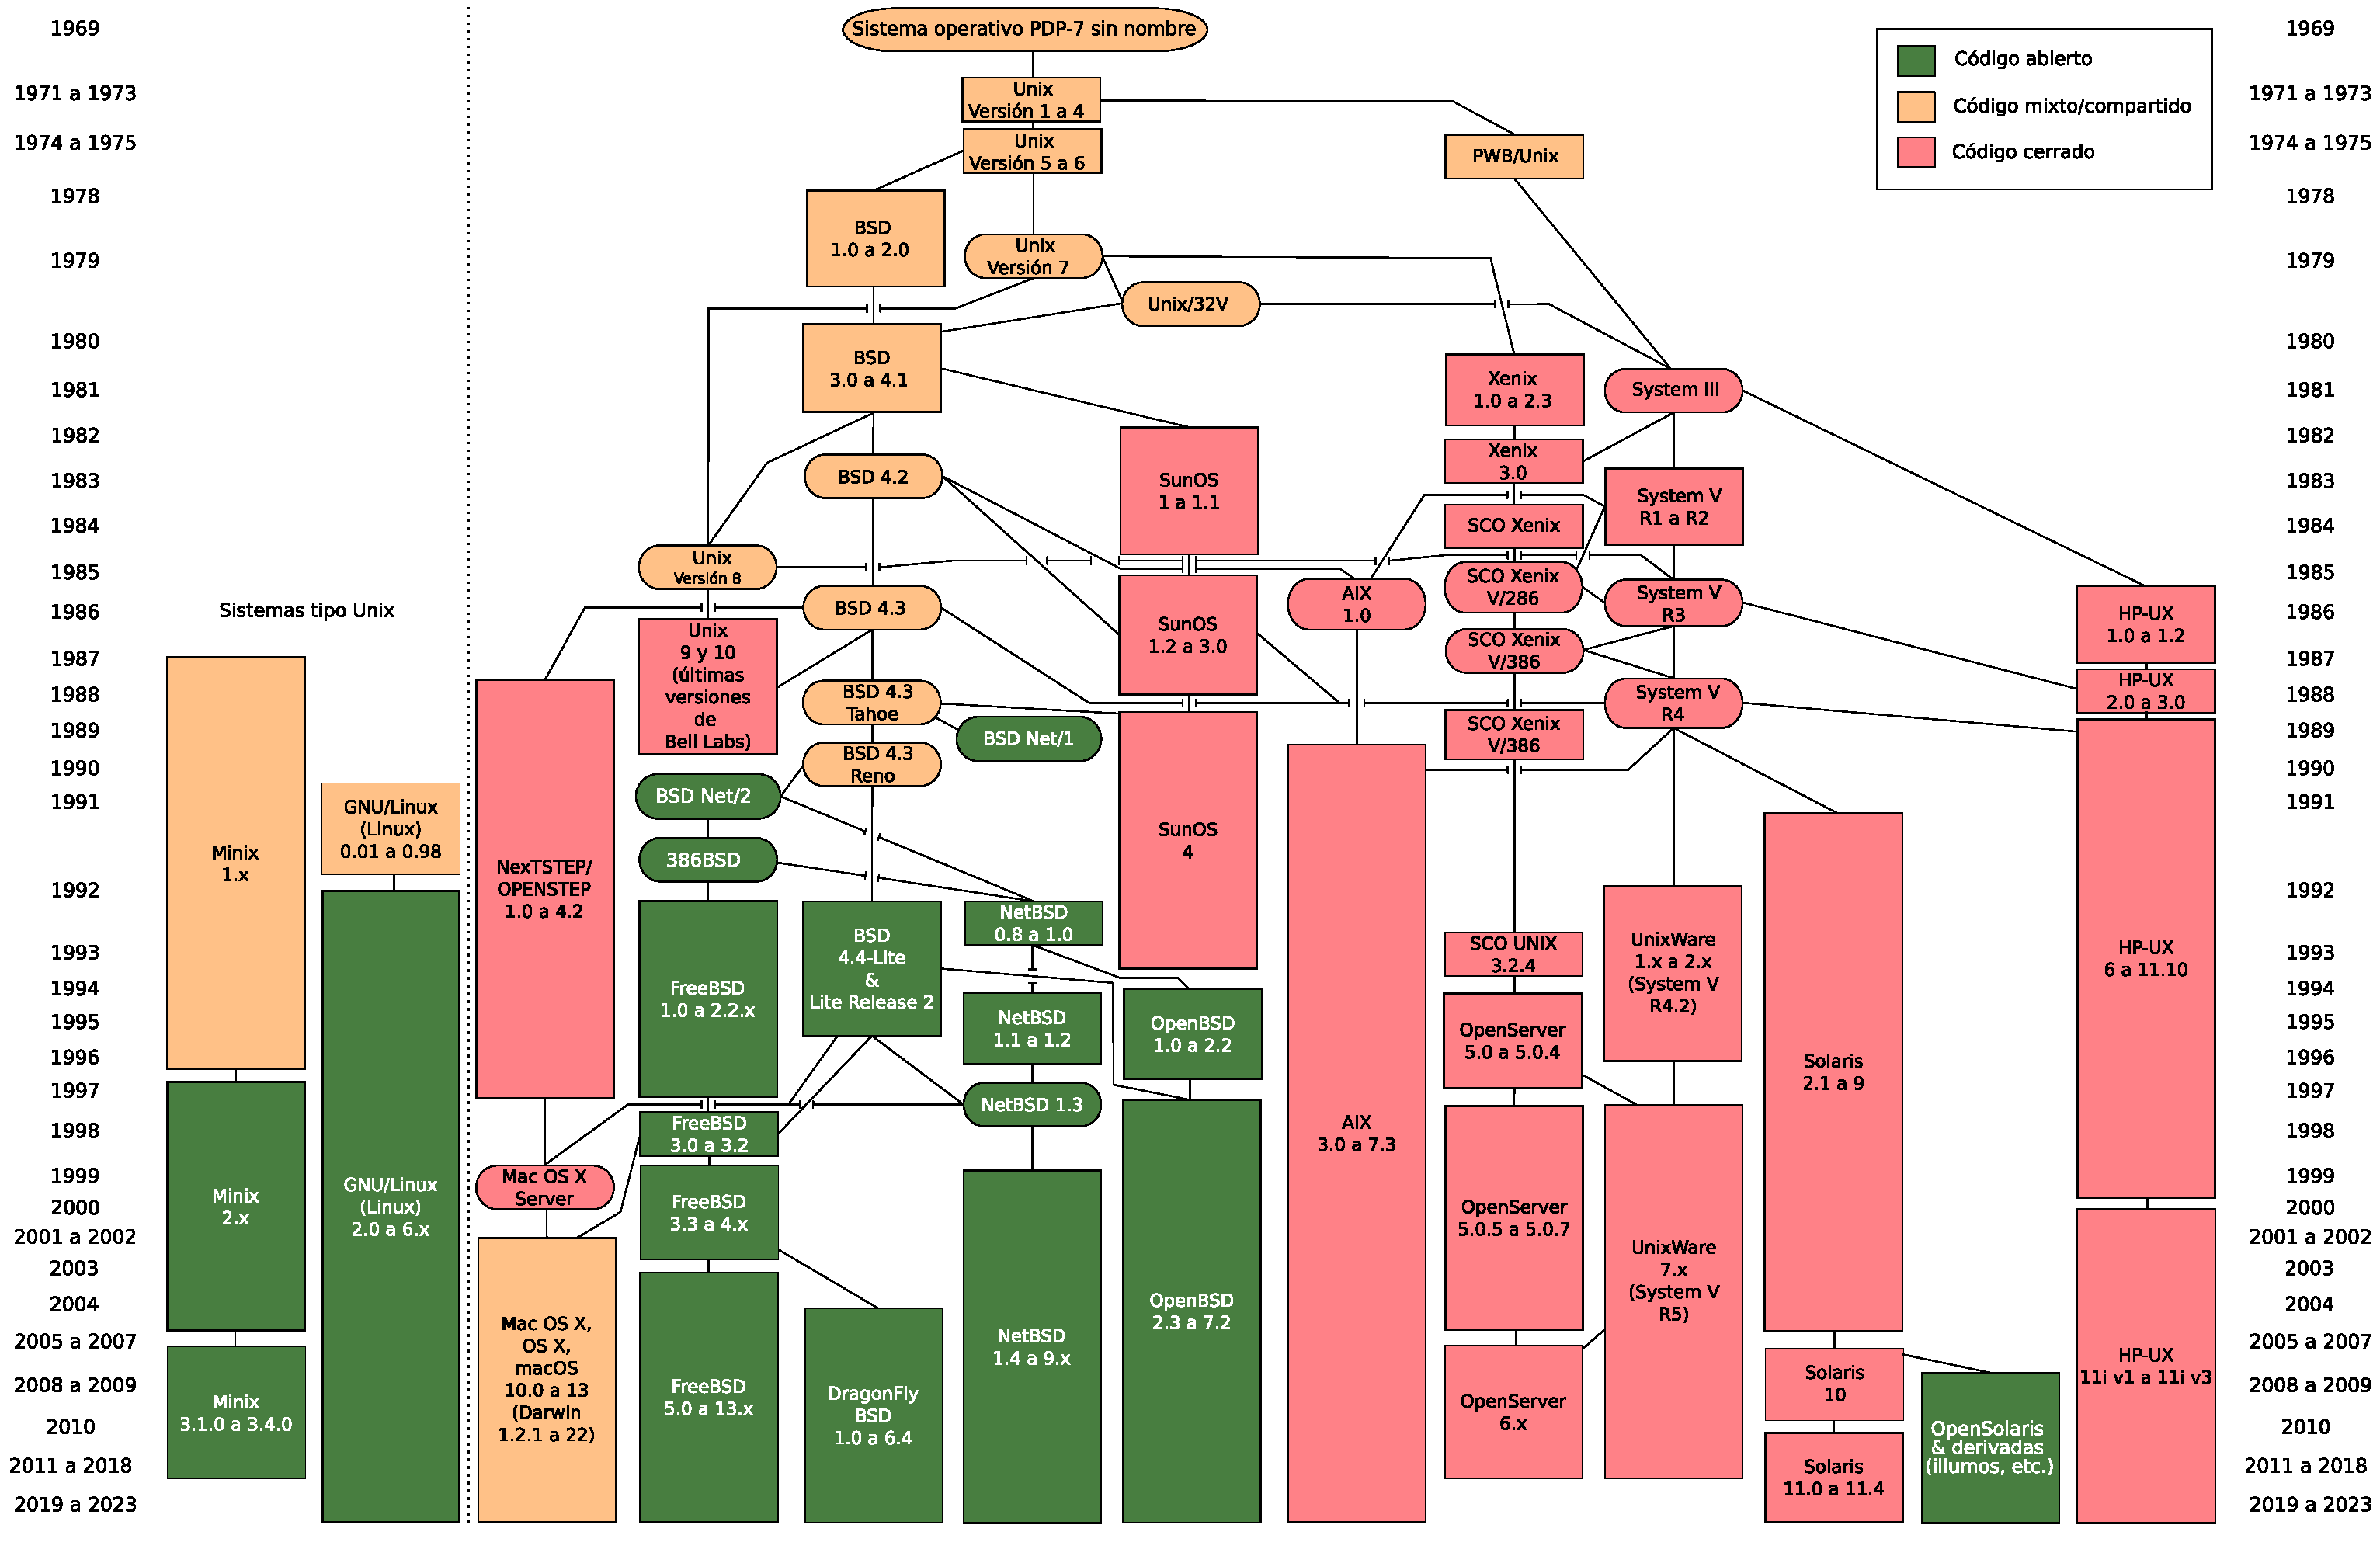
\includegraphics[width=1\textwidth]{figs/unix_tree_vector.pdf}
  \figsource{\getauthor{unix_family_tree}, \gettitle{unix_family_tree} (\getyear{unix_family_tree})~\cite{unix_family_tree}.}
  \caption{Árbol genealógico de los sistemas operativos \textit{Unix}.}
  \label{fig:unix_tree}
\end{figure}

Como ilustra la imagen anterior, \textit{Unix} es el sistema pionero creado en los años 70 que sentó las bases de la informática e inspiró directamente el desarrollo de \textit{Linux}, desarrollado íntegramente bajo un modelo de código abierto. También \textit{macOS} proviene de esta familia; sin embargo, este sistema operativo ha evolucionado bajo un modelo comercial semi-privativo y de código parcialmente cerrado.\\

La hegemonía de \textit{GNU/Linux} en estos sectores se debe principalmente a su filosofía de código abierto (\textit{open-source}). Disponer del código fuente de manera pública, ya sea mediante la instalación local de cabeceras y fuentes del sistema (típicamente situados en entornos de desarrollo en \texttt{/usr/src}) o en repositorios públicos en línea (\textit{GitHub}), permite a una gran comunidad mundial de desarrolladores auditar, depurar y mejorar el código del mismo de forma continua.
Esta transparencia garantiza un nivel de adaptabilidad y fiabilidad muy superior al de los sistemas comerciales, permitiendo una configuración del entorno a medida según las necesidades requeridas.\\

Por estos motivos, se considera \textit{GNU/Linux} el sistema operativo óptimo para desarrollar este proyecto. Por consiguiente, a partir de este punto se asumirá por defecto que nos encontramos en un entorno \textit{Linux}.

\

\

\subsection{Arquitectura y anillos de privilegios}
\label{sec:estructuralinux}

Para garantizar su estabilidad y seguridad, los sistemas operativos modernos no confían únicamente en restricciones lógicas de \textit{software}, sino que se apoyan de forma entrelazada en mecanismos de protección implementados a nivel de \textit{hardware} por el propio procesador.
En arquitecturas de sistemas predominantes como la familia x86, este mecanismo de aislamiento se implementa típicamente a través de dominios concéntricos de protección jerárquicos, comúnmente conocidos como anillos de protección (\textit{Protection Rings})~\cite{librossoo}.\\

\begin{figure}[h!]
  \centering
  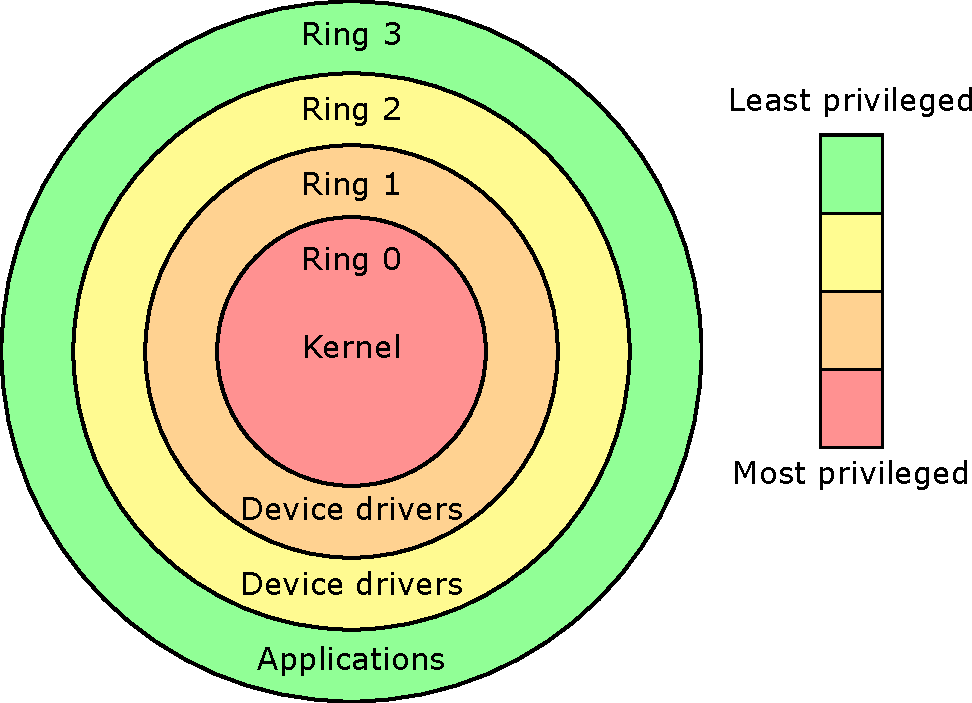
\includegraphics[width=0.65\textwidth]{figs/rings.pdf}
  \figsource{\getauthor{wiki_rings}, \gettitle{wiki_rings} (\getyear{wiki_rings})~\cite{wiki_rings}.}
  \caption{Anillos de privilegios en sistemas operativos modernos.}
  \label{fig:protection_rings}
\end{figure}

Esta arquitectura determina principalmente cuatro niveles de privilegios concéntricos, comúnmente llamados ``anillos'', numerados del 0 al 3. El nivel de privilegio implica qué instrucciones de la CPU puede ejecutar un proceso y a qué regiones de la memoria puede acceder al ejecutarse, distinguiendo estos cuatro anillos~\cite{librossoo}:

\begin{itemize}
    \item \textbf{\textit{Ring 0}:} Nivel de máximo privilegio, donde reside típicamente el núcleo (\textit{kernel}). Los programas ejecutados en este anillo tienen prácticamente acceso directo e irrestricto a todo el \textit{hardware}, la memoria y las instrucciones del procesador.
    \item \textbf{\textit{Ring 1 y 2}:} Originalmente diseñados para servicio y control del propio sistema con privilegios intermedios, aunque en la práctica han sido mayormente descartados por la mayoría de sistemas operativos, debido a su complejidad y bajo rendimiento.
    \item \textbf{\textit{Ring 3}:} Nivel de menor privilegio. Los procesos lanzados en este anillo no pueden interactuar directamente con el \textit{hardware}, debiendo delegar cualquier operación crítica a niveles de mayor privilegio.
\end{itemize}

Por motivos de eficiencia y portabilidad a otras arquitecturas de procesadores (como \textit{ARM}, que normalmente no posee tantos niveles), \textit{Linux} simplifica este modelo y utiliza exclusivamente dos de estos anillos.
Por un lado, se aísla el \textit{kernel} (núcleo del sistema), ejecutándolo íntegramente en el \textit{Ring 0}, y por otro lado, se confina el resto de programas de usuario en la región del \textit{Ring 3}~\cite{love_linux, librossoo}.\\

\begin{figure}[h!]
  \centering
  \scalebox{1.1}{\definecolor{osouter}{RGB}{235, 226, 192}
\definecolor{oslibs}{RGB}{238, 224, 145}
\definecolor{oskernel}{RGB}{239, 180, 141}
\definecolor{oshw}{RGB}{255, 110, 0}
\definecolor{ostext}{RGB}{25, 25, 25}

\begin{tikzpicture}[
  x=1cm,
  y=1cm,
  box/.style={draw=black, line width=0.8pt},
  biglabel/.style={font=\fontfamily{Inter-LF}\fontsize{9}{10}\selectfont, text=ostext},
  ringlabel/.style={font=\fontfamily{Inter-LF}\itshape\fontsize{8}{9}\selectfont, text=ostext},
  leftlabel/.style={font=\fontfamily{Inter-LF}\fontsize{9}{10}\selectfont, text=ostext, anchor=east}
]

  % Main stacked architecture
  \fill[osouter] (3.95, 0.45) rectangle (11.05, 6.85);
  \draw[box] (3.95, 0.45) rectangle (11.05, 6.85);

  \fill[oslibs] (3.95, 2.10) rectangle (10.25, 5.90);
  \draw[box] (3.95, 2.10) rectangle (10.25, 5.90);

  \fill[oskernel] (3.95, 2.10) rectangle (9.42, 4.98);
  \draw[box] (3.95, 2.10) rectangle (9.42, 4.98);

  \fill[oshw] (3.95, 0.45) rectangle (11.05, 2.10);
  \draw[box] (3.95, 0.45) rectangle (11.05, 2.10);

  % Left-side annotations
  \node[leftlabel] at (3.82, 5.92) {API, programming interface};
  \node[leftlabel] at (3.82, 4.98) {System calls};
  \node[leftlabel] at (3.82, 2.15) {ISA, architecture instructions};

  % Outer user area / application
  \node[biglabel, anchor=east] at (11.1, 6.5) {Application};
  \node[ringlabel, anchor=east] at (11.1, 6.20) {User area (ring 3)};

  % Libraries
  \node[biglabel, anchor=east] at (10.3, 5.6) {Libraries};
  \node[ringlabel, anchor=east] at (10.3, 5.3) {User area (ring 3)};

  % Kernel
  \node[biglabel, anchor=east] at (9.5, 3.85) {Operating System};
  \node[ringlabel, anchor=east] at (9.5, 3.50) {Kernel (ring 0)};

  % Hardware
  \node[biglabel, anchor=east] at (10.5, 1.30) {Hardware (CPU)};

\end{tikzpicture}
}
  \figsource{\getauthor{librossoo}, \gettitle{librossoo} (\getyear{librossoo})~\cite{librossoo}.}
  \caption{Estructura de un sistema operativo moderno.}
  \label{fig:os_structure}
\end{figure}

Básicamente, la estructura del sistema operativo se puede describir como una división física de privilegios que se traduce directamente en una arquitectura lógica estructurada en capas construidas unas encima de otras~\cite{librossoo}.\\

En la base se encuentra el \textit{hardware} físico de la máquina, con el cual el núcleo interactúa directamente a través de las instrucciones de la arquitectura (ISA) disponibles.
Inmediatamente por encima, operando con privilegios absolutos sobre el sistema, en el \textit{Ring 0}, reside el \textit{kernel}. Este es el corazón del sistema operativo, responsable de gestionar los recursos de la máquina y de actuar como puente fundamental entre el \textit{hardware} y las aplicaciones de usuario.
Posteriormente, en las capas más externas del mismo, se encuentran las bibliotecas del sistema, encargadas de proporcionar la \textbf{\textit{interfaz de programación de aplicaciones (API)}}, y las aplicaciones finales, las cuales se encuentran confinadas en el área de usuario (\textit{Ring~3}).\\

Debido a esta separación, si algún proceso de esta región de usuario requiere realizar una acción privilegiada (como leer un archivo del disco, enviar un paquete de red o reservar memoria), no puede acceder al \textit{hardware} directamente por sí mismo.
En su lugar, debe solicitar dicha operación privilegiada al \textit{kernel} atravesando la frontera del \textit{Ring~0} mediante un mecanismo de comunicación estandarizado y controlado, comúnmente conocido como \textbf{\textit{llamadas al sistema}} (\textit{System Calls} o \textit{syscalls}).\\

Esta barrera arquitectónica no solo define qué instrucciones se pueden ejecutar y dónde, sino que obliga al sistema operativo a dividir la memoria principal de rápido acceso (\textit{RAM}) en dos grandes regiones virtuales completamente aisladas en \textbf{\textit{espacio de usuario}} y \textbf{\textit{espacio de kernel}},
garantizando así controlar que ningún proceso de usuario pueda corromper datos sensibles internos del sistema~\cite{love_linux, librossoo}.

\

\

\subsection{Memoria: Espacio de usuario y espacio de kernel}
\label{sec:uskrspaces}

Para comprender cómo se materializa la división de privilegios descrita en el apartado anterior realmente en la memoria física de la máquina (\textit{RAM}), es necesario introducir el concepto de \textit{memoria virtual}.\\

En los sistemas \textit{Linux} modernos, los procesos no acceden directamente a las direcciones físicas de la memoria \textit{RAM}.
En su lugar, el \textit{kernel} y la unidad de gestión de memoria (\textit{MMU}) de la \textit{CPU} proporcionan a cada proceso la ilusión de tener espacio exclusivo y contiguo a través de la \textbf{\textit{memoria virtual}}.
Para lograrlo, la \textit{MMU} traduce dinámicamente las direcciones virtuales de memoria a ubicaciones físicas reales y viceversa, consultando una \textbf{\textit{tabla de páginas}}.
De esta forma, se garantiza que múltiples procesos puedan ejecutarse simultáneamente de forma aislada y segura, cada uno con su propio mapa de direcciones gestionado íntegramente por el \textit{kernel}~\cite{silberschatz_memoria}.\\

A su vez, este espacio de \textit{memoria virtual} se divide de forma estricta en dos grandes regiones, fuertemente relacionadas con la arquitectura de anillos de protección del procesador:

\begin{itemize}
    \item \textbf{Espacio de Usuario (\textit{User Space}):} Es la porción inferior de la memoria virtual, asociada al \textit{Ring 3}. En esta región se cargan y ejecutan las aplicaciones de usuario, sus bibliotecas y los datos pertinentes.
    Si un proceso comete un error ``crítico'' en esta región (como intentar acceder a memoria que no le pertenece), el sistema operativo interviene para finalizar dicho proceso y genera un error (típicamente conocido como \textit{Segmentation Fault}), evitando que el fallo afecte al resto del sistema.
    \item \textbf{Espacio del Kernel (\textit{Kernel Space}):} Es la porción superior de la memoria virtual, reservada exclusivamente para el \textbf{\textit{kernel}} con sus módulos y los controladores de dispositivos (\textit{drivers}).
    Al estar asociado al \textit{Ring 0}, el código que reside aquí tiene acceso total a la memoria física y, por consiguiente, al \textit{hardware}. Un fallo de programación o una intrusión maliciosa en este nivel compromete todo el sistema, pudiendo provocar una caída total del mismo (\textit{Kernel Panic}).
\end{itemize}

\begin{figure}[h!]
  \centering
  \scalebox{0.65}{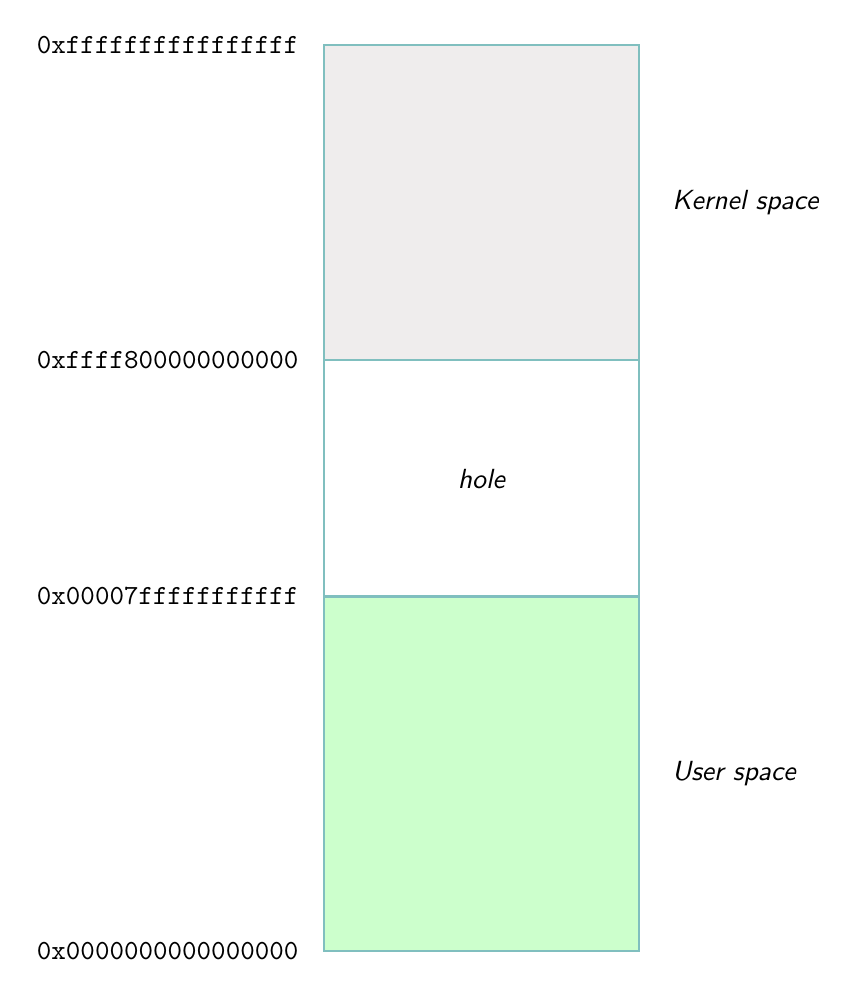
\begin{tikzpicture}[
    % Estilos de las cajas (colores suaves mezclados)
    userbox/.style={thick, draw=teal!50, fill=green!20},
    holebox/.style={thick, draw=teal!50, fill=white},
    kernelbox/.style={thick, draw=teal!50, fill=pink!15!gray!15},
    % Estilos para los textos
    addr/.style={font=\ttfamily, text=black, anchor=east},
    labeltext/.style={font=\sffamily\itshape, text=black, anchor=west}
]

% --- USER SPACE ---
\draw[userbox] (0, 0) rectangle (4, 4.5);
\node[labeltext] (user) at (4.3, 2.25) {User space};
\node[addr] (addr1) at (-0.2, 0) {0x0000000000000000};
\node[addr] (addr2) at (-0.2, 4.5) {0x00007fffffffffff};

% --- HOLE ---
\draw[holebox] (0, 4.5) rectangle (4, 7.5);
\node[font=\sffamily\itshape, text=black] (hole) at (2, 6) {hole};

% --- KERNEL SPACE ---
\draw[kernelbox] (0, 7.5) rectangle (4, 11.5);
\node[labeltext] (kernel) at (4.3, 9.5) {Kernel space};
\node[addr] (addr3) at (-0.2, 7.5) {0xffff800000000000};
\node[addr] (addr4) at (-0.2, 11.5) {0xffffffffffffffff};

\end{tikzpicture}}
  \figsource{\getauthor{librossoo}, \gettitle{librossoo} (\getyear{librossoo})~\cite{librossoo}.}
  \caption{División lógica de memoria en Espacio de Usuario y Espacio del Kernel.}
  \label{fig:usr_krn_memory}
\end{figure}

De la misma manera que la \textit{memoria virtual} abstrae la complejidad de organización de la memoria física (\textit{RAM}) para garantizar el aislamiento y la ejecución segura de los procesos,
el sistema operativo proporciona a su vez una abstracción equivalente para la gestión del almacenamiento persistente y la interacción con el resto de componentes del sistema.
Esta importante tarea recae sobre otro gran pilar estructural de un sistema operativo, en este caso \textit{Linux}: su \textit{sistema de ficheros} (\textit{file system}).

\

\

\subsection{Ficheros y Sistemas de Ficheros (\textit{FS})}
\label{sec:fs}

Una de las características más destacadas de la arquitectura de \textit{Linux}, heredada directamente de la familia original de \textit{Unix}, es el principio fundamental de que \guillemotleft todo es un fichero\guillemotright.
En este tipo de sistemas operativos, no solo los documentos de texto o los programas ejecutables binarios son tratados como ficheros, sino también los directorios, las conexiones de red (\textit{sockets}), los dispositivos de \textit{hardware} (como terminales o discos duros),
así como la información dinámica de los procesos en ejecución y del propio sistema (como los ficheros virtuales situados en el directorio \texttt{/proc})~\cite{love_linux}.\\

Para estructurar, acceder y organizar toda esta enorme cantidad de información, el sistema operativo emplea un \textbf{Sistema de Ficheros (\textit{FS})}, el cual se puede definir como el conjunto de reglas, métodos y jerarquías lógicas encargados de gestionar cómo los ficheros se nombran, se almacenan y se recuperan en un medio lógico.\\

Debido a la gran cantidad de datos y recursos tanto físicos como lógicos que maneja la máquina, es necesario mantener un orden universal de los mismos para que el sistema operativo sepa exactamente dónde se encuentran.
Como solución a esta necesidad organizativa, \textit{Linux} adopta el estándar \textbf{\textit{FHS} (\textit{Filesystem Hierarchy Standard})}, que define una jerarquía global de directorios raíz donde se distribuyen los distintos tipos de ficheros del sistema, como binarios, bibliotecas, ficheros de configuración, datos persistentes y recursos dinámicos, según su función, tipo y alcance.\\

\begin{figure}[H]
  \centering
  \scalebox{0.8}{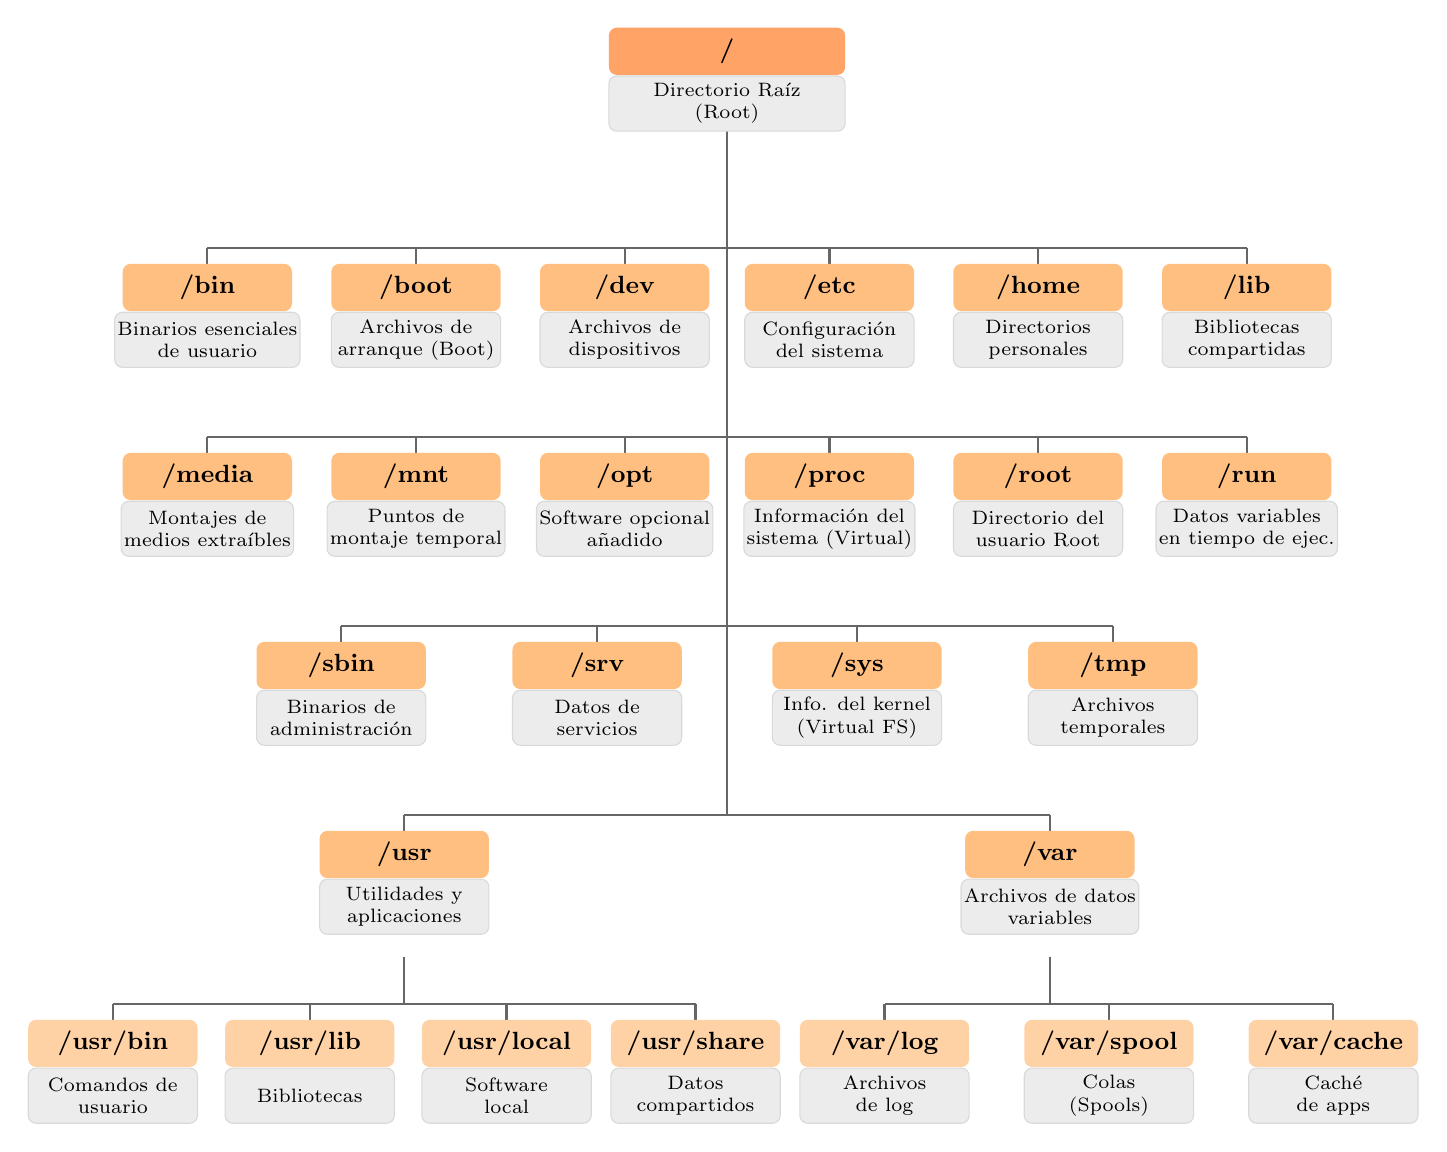
\begin{tikzpicture}[
    % Estilos de las cajas (carpetas y descripciones)
    dir/.style={fill=#1, text=black, font=\bfseries\small, minimum width=2.15cm, minimum height=0.6cm, rounded corners=1mm, inner sep=0pt},
    desc/.style={fill=gray!15, draw=gray!30, text=black, font=\scriptsize, align=center, minimum width=2.15cm, minimum height=0.7cm, rounded corners=1mm, anchor=north, inner sep=1pt},
    treeline/.style={thick, draw=gray!80!black}
]

% ---------------------------------------------------------
% 1. LÍNEAS DEL ÁRBOL (Estructura de conexión)
% ---------------------------------------------------------
% Tronco central (Estirado hacia arriba para conectar con el nuevo Raíz)
\draw[treeline] (0, 0.5) -- (0, -8.2);

% Fila 1 (Tier 1)
\draw[treeline] (-6.6, -1.0) -- (6.6, -1.0);
\foreach \x in {-6.6, -3.95, -1.3, 1.3, 3.95, 6.6} \draw[treeline] (\x, -1.0) -- (\x, -1.5);

% Fila 2 (Tier 2)
\draw[treeline] (-6.6, -3.4) -- (6.6, -3.4);
\foreach \x in {-6.6, -3.95, -1.3, 1.3, 3.95, 6.6} \draw[treeline] (\x, -3.4) -- (\x, -3.9);

% Fila 3 (Tier 3)
\draw[treeline] (-4.9, -5.8) -- (4.9, -5.8);
\foreach \x in {-4.9, -1.65, 1.65, 4.9} \draw[treeline] (\x, -5.8) -- (\x, -6.3);

% Fila 4 (Tier 4) - usr y var
\draw[treeline] (-4.1, -8.2) -- (4.1, -8.2);
\foreach \x in {-4.1, 4.1} \draw[treeline] (\x, -8.2) -- (\x, -8.7);

% Sub-árbol de /usr
\draw[treeline] (-4.1, -10.0) -- (-4.1, -10.6);
\draw[treeline] (-7.8, -10.6) -- (-0.4, -10.6);
\foreach \x in {-7.8, -5.3, -2.8, -0.4} \draw[treeline] (\x, -10.6) -- (\x, -11.1);

% Sub-árbol de /var
\draw[treeline] (4.1, -10.0) -- (4.1, -10.6);
\draw[treeline] (2.0, -10.6) -- (7.7, -10.6);
\foreach \x in {2.0, 4.85, 7.7} \draw[treeline] (\x, -10.6) -- (\x, -11.1);


% ---------------------------------------------------------
% 2. CAJAS Y TEXTOS (Nodos)
% ---------------------------------------------------------
% ROOT (Elevado a y=1.5 para darle aire y jerarquía)
\node[dir=orange!80!red!60, minimum width=3cm] (root) at (0, 1.5) {/};
\node[desc, minimum width=3cm] at (root.south) {Directorio Raíz\\(Root)};

% --- FILA 1 ---
\node[dir=orange!50] (bin) at (-6.6, -1.5) {/bin};
\node[desc] at (bin.south) {Binarios esenciales\\de usuario};

\node[dir=orange!50] (boot) at (-3.95, -1.5) {/boot};
\node[desc] at (boot.south) {Archivos de\\arranque (Boot)};

\node[dir=orange!50] (dev) at (-1.3, -1.5) {/dev};
\node[desc] at (dev.south) {Archivos de\\dispositivos};

\node[dir=orange!50] (etc) at (1.3, -1.5) {/etc};
\node[desc] at (etc.south) {Configuración\\del sistema};

\node[dir=orange!50] (home) at (3.95, -1.5) {/home};
\node[desc] at (home.south) {Directorios\\personales};

\node[dir=orange!50] (lib) at (6.6, -1.5) {/lib};
\node[desc] at (lib.south) {Bibliotecas\\compartidas};

% --- FILA 2 ---
\node[dir=orange!50] (media) at (-6.6, -3.9) {/media};
\node[desc] at (media.south) {Montajes de\\medios extraíbles};

\node[dir=orange!50] (mnt) at (-3.95, -3.9) {/mnt};
\node[desc] at (mnt.south) {Puntos de\\montaje temporal};

\node[dir=orange!50] (opt) at (-1.3, -3.9) {/opt};
\node[desc] at (opt.south) {Software opcional\\añadido};

\node[dir=orange!50] (proc) at (1.3, -3.9) {/proc};
\node[desc] at (proc.south) {Información del\\sistema (Virtual)};

\node[dir=orange!50] (rootdir) at (3.95, -3.9) {/root};
\node[desc] at (rootdir.south) {Directorio del\\usuario Root};

\node[dir=orange!50] (run) at (6.6, -3.9) {/run};
\node[desc] at (run.south) {Datos variables\\en tiempo de ejec.};

% --- FILA 3 ---
\node[dir=orange!50] (sbin) at (-4.9, -6.3) {/sbin};
\node[desc] at (sbin.south) {Binarios de\\administración};

\node[dir=orange!50] (srv) at (-1.65, -6.3) {/srv};
\node[desc] at (srv.south) {Datos de\\servicios};

\node[dir=orange!50] (sys) at (1.65, -6.3) {/sys};
\node[desc] at (sys.south) {Info. del kernel\\(Virtual FS)};

\node[dir=orange!50] (tmp) at (4.9, -6.3) {/tmp};
\node[desc] at (tmp.south) {Archivos\\temporales};

% --- FILA 4 (Nodos padres de expansión) ---
\node[dir=orange!50] (usr) at (-4.1, -8.7) {/usr};
\node[desc] at (usr.south) {Utilidades y\\aplicaciones};

\node[dir=orange!50] (var) at (4.1, -8.7) {/var};
\node[desc] at (var.south) {Archivos de datos\\variables};

% --- FILA 5 (Hijos de /usr) ---
\node[dir=orange!35] (usrbin) at (-7.8, -11.1) {/usr/bin};
\node[desc] at (usrbin.south) {Comandos de\\usuario};

\node[dir=orange!35] (usrlib) at (-5.3, -11.1) {/usr/lib};
\node[desc] at (usrlib.south) {Bibliotecas};

\node[dir=orange!35] (usrlocal) at (-2.8, -11.1) {/usr/local};
\node[desc] at (usrlocal.south) {Software\\local};

\node[dir=orange!35] (usrshare) at (-0.4, -11.1) {/usr/share};
\node[desc] at (usrshare.south) {Datos\\compartidos};

% --- FILA 5 (Hijos de /var) ---
\node[dir=orange!35] (varlog) at (2.0, -11.1) {/var/log};
\node[desc] at (varlog.south) {Archivos\\de log};

\node[dir=orange!35] (varspool) at (4.85, -11.1) {/var/spool};
\node[desc] at (varspool.south) {Colas\\(Spools)};

\node[dir=orange!35] (varcache) at (7.7, -11.1) {/var/cache};
\node[desc] at (varcache.south) {Caché\\de apps};

\end{tikzpicture}
}
  \figsource{Elaboración propia basada en \getauthor{albritton_fs}, ``\gettitle{albritton_fs}'' (\getyear{albritton_fs})~\cite{albritton_fs}.}
  \caption{Estructura jerárquica estándar de directorios en \textit{Linux} (\textit{FHS}).}
  \label{fig:fhs}
\end{figure}

Dentro de esta estructura, uno de los directorios más singulares es \texttt{/proc}, ya que no almacena datos persistentes en disco, sino que constituye un pseudo-sistema de ficheros generado dinámicamente por el \textit{kernel} en memoria (\textit{RAM}) mediante \textbf{ficheros virtuales}.
Su principal propósito es exponer, a través de una interfaz basada en ficheros, información sobre parámetros del sistema, procesos en ejecución y determinados estados internos del \textit{kernel}, como \texttt{/proc/meminfo} o \texttt{/proc/cpuinfo}.
El acceso a estas entradas se realiza mediante operaciones estándar sobre ficheros, como \texttt{read()} o \texttt{write()}, que el \textit{kernel} redirige a los manejadores correspondientes según la naturaleza y propósito de cada fichero virtual.

De esta manera, es posible crear interfaces de comunicación entre el \textit{Espacio de Usuario} y el \textit{Espacio del Kernel} mediante \textit{Módulos del Kernel} que creen nuevas entradas de fichero virtual dentro de este directorio,
permitiendo asociar operaciones de lectura y escritura a manejadores específicos para solicitar o reportar información sensible del sistema de forma controlada.\\

Para gestionar esta gran heterogeneidad de recursos y permitir la coexistencia de múltiples sistemas de ficheros físicos (como \textit{ext4} o \textit{NTFS}) en un mismo sistema anfitrión, el \textit{kernel} implementa una capa de abstracción denominada \textbf{Sistema de Ficheros Virtual (\textit{VFS})},
situada entre la capa de llamadas al sistema (\textit{syscalls}) y los \textit{drivers} de bajo nivel.
Su función es proporcionar una \textit{API} unificada que permite a las aplicaciones del \textit{Espacio de Usuario} utilizar llamadas estándar (como \texttt{read()} o \texttt{write()}) sobre cualquier fichero o dispositivo, abstrayendo por completo los detalles del \textit{hardware} de la máquina~\cite{librossoo}.\\

\begin{figure}[h!]
  \centering
  \scalebox{0.8}{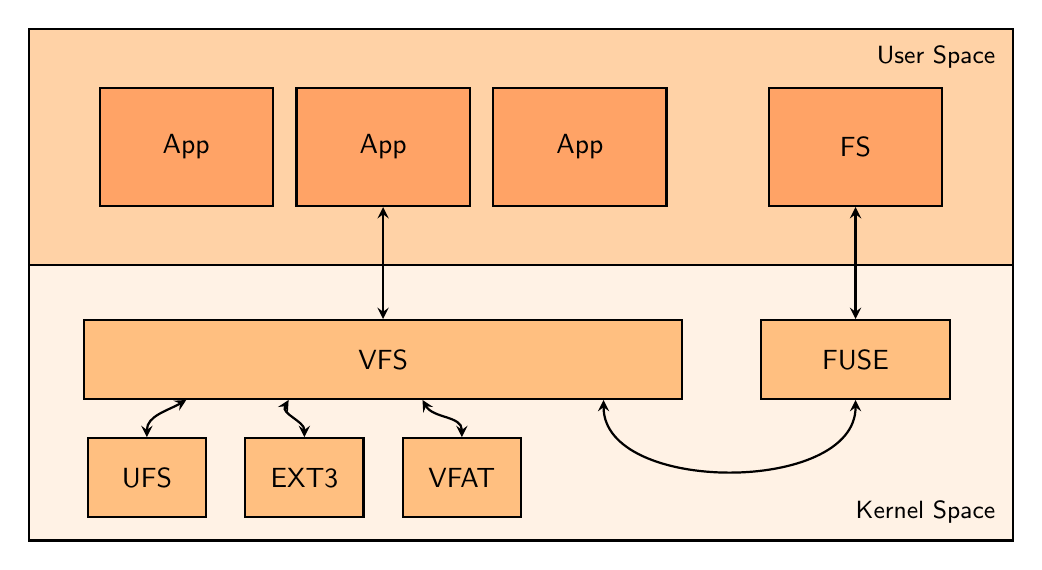
\begin{tikzpicture}[
    % Estilos de colores y cajas para clavarlo a tu imagen
    userbg/.style={fill=orange!35, thick, draw=black},
    kernelbg/.style={fill=orange!10, thick, draw=black},
    appbox/.style={draw=black, thick, fill=orange!80!red!60, minimum width=2.2cm, minimum height=1.5cm, font=\sffamily},
    kernelbox/.style={draw=black, thick, fill=orange!50, minimum height=1cm, font=\sffamily},
    arrow/.style={<->, thick, >=stealth}
]

% 1. Fondos (Cajas grandes de área)
\draw[kernelbg] (0, 0) rectangle (12.5, 3.5);
\draw[userbg] (0, 3.5) rectangle (12.5, 6.5);

% 2. Textos de las áreas (Modified label for User Space)
\node[anchor=north east, font=\sffamily\small] at (12.4, 6.4) {User Space}; % Changed to English, same position

% 3. Cajas del Área de Usuario (Naranja oscuro)
\node[appbox] (app1) at (2, 5) {App};
\node[appbox] (app2) at (4.5, 5) {App};
\node[appbox] (app3) at (7, 5) {App};
\node[appbox] (fs)   at (10.5, 5) {FS};

% 4. Cajas del Área de Kernel (Naranja claro)
\node[kernelbox, minimum width=7.6cm] (vfs) at (4.5, 2.3) {VFS};
\node[kernelbox, minimum width=2.4cm] (fuse) at (10.5, 2.3) {FUSE};

\node[kernelbox, minimum width=1.5cm] (ufs)  at (1.5, 0.8) {UFS};
\node[kernelbox, minimum width=1.5cm] (ext3) at (3.5, 0.8) {EXT3};
\node[kernelbox, minimum width=1.5cm] (vfat) at (5.5, 0.8) {VFAT};

% New English Kernel Space label, tucked neatly into the bottom-right corner *inside* the box
\node[anchor=south east, font=\sffamily\small] at (12.4, 0.1) {Kernel Space}; % Changed to English, new position

% 5. Flechas verticales rectas
\draw[arrow] (app2.south) -- (vfs.north);
\draw[arrow] (fs.south) -- (fuse.north);

% 6. Flechas inferiores curvas hacia VFS
\draw[arrow] (ufs.north) to[out=90, in=210] ([xshift=-2.5cm]vfs.south);
\draw[arrow] (ext3.north) to[out=90, in=240] ([xshift=-1.2cm]vfs.south);
\draw[arrow] (vfat.north) to[out=90, in=300] ([xshift=0.5cm]vfs.south);

% 7. Flecha curva larga (de VFS a FUSE)
\draw[arrow] ([xshift=2.8cm]vfs.south) .. controls +(down:1.2) and +(down:1.2) .. (fuse.south);

\end{tikzpicture}}
  \figsource{\getauthor{librossoo}, \gettitle{librossoo} (\getyear{librossoo})~\cite{librossoo}.}
  \caption{Gestión de sistemas de ficheros en \textit{Linux}.}
  \label{fig:vfs}
\end{figure}

Principalmente, el \textit{VFS} actúa como un enrutador central entre el \textit{Espacio de Usuario} y el \textit{Espacio del Kernel}, recibiendo las peticiones de las aplicaciones y redirigiéndolas de forma transparente al \textit{driver} físico correspondiente.
Además, los sistemas modernos soportan mecanismos avanzados como \textit{FUSE} (\textit{Filesystem in Userspace}), que permite al \textit{VFS} delegar la gestión de ciertos sistemas de ficheros a procesos que se ejecutan de forma segura directamente en el \textit{Espacio de Usuario}.\\

Para integrar distintos sistemas de ficheros dentro del sistema anfitrión, \textit{Linux} prescinde de unidades aisladas y utiliza la tecnología de \textbf{montaje} (\textit{mounting}).
Este mecanismo unificador ``engancha'' lógicamente cualquier sistema de ficheros externo a un directorio existente (típicamente \texttt{/mnt} o \texttt{/media}), considerado \textbf{punto de montaje} (\textit{mount point}).
De este modo, se crea una estructura de directorios continua y transparente que abstrae al usuario de la naturaleza del medio externo subyacente~\cite{love_linux}.\\

\begin{figure}[h!]
  \centering
  \scalebox{0.8}{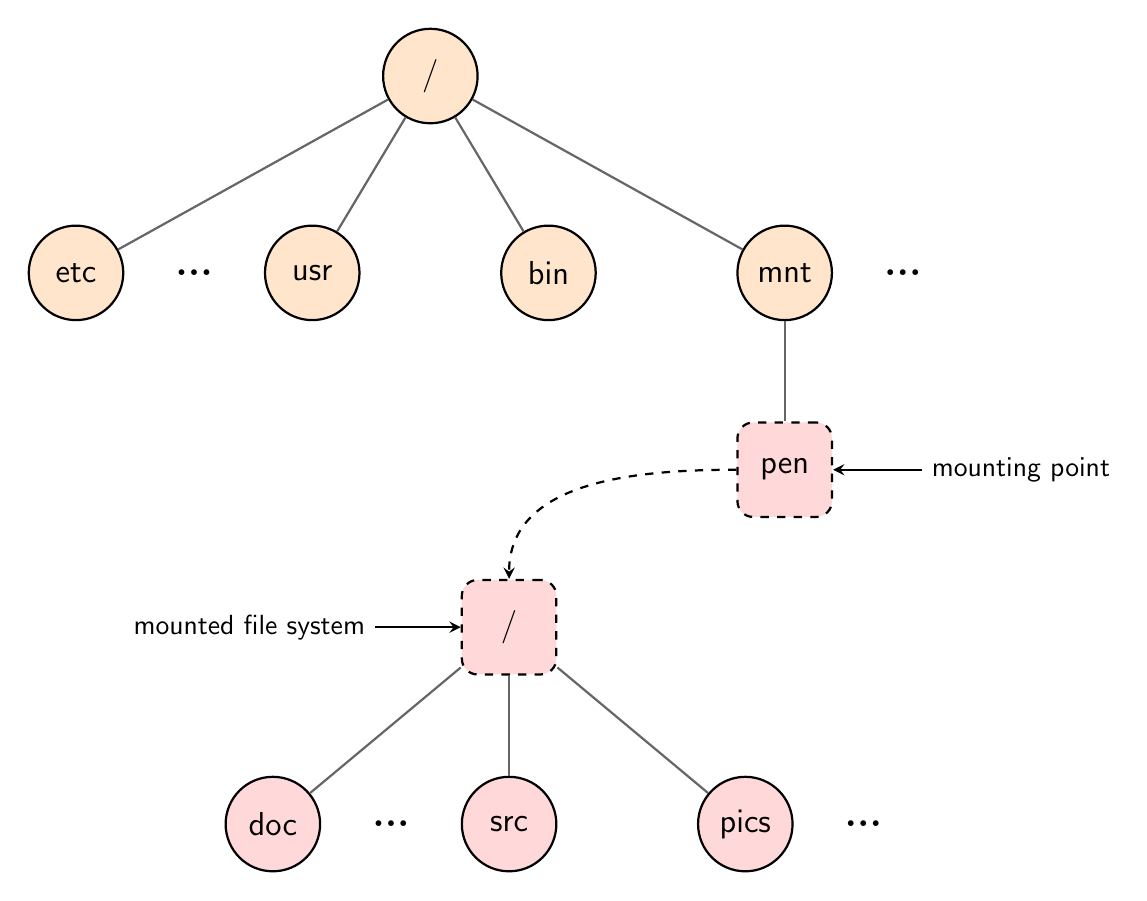
\begin{tikzpicture}[
    % Estilos de los nodos (colores suaves como en tu imagen)
    mainfs/.style={circle, draw=black, thick, fill=orange!20, minimum size=1.2cm, font=\sffamily\large},
    mountfs/.style={circle, draw=black, thick, fill=red!15, minimum size=1.2cm, font=\sffamily\large},
    mountbox/.style={rectangle, rounded corners=2mm, draw=black, thick, dashed, fill=red!15, minimum size=1.2cm, font=\sffamily\large},
    texto/.style={font=\sffamily, text=black},
    line/.style={-, thick, draw=gray!80!black},
    arrow/.style={->, thick, >=stealth, draw=black}
]

% --- SISTEMA DE FICHEROS PRINCIPAL ---
\node[mainfs] (root1) at (0, 0) {/};

\node[mainfs] (etc) at (-4.5, -2.5) {etc};
\node[font=\bfseries\Large] at (-3, -2.5) {...};
\node[mainfs] (usr) at (-1.5, -2.5) {usr};
\node[mainfs] (bin) at (1.5, -2.5) {bin};
\node[mainfs] (mnt) at (4.5, -2.5) {mnt};
\node[font=\bfseries\Large] at (6, -2.5) {...};

\draw[line] (root1) -- (etc);
\draw[line] (root1) -- (usr);
\draw[line] (root1) -- (bin);
\draw[line] (root1) -- (mnt);

% --- PUNTO DE MONTAJE (pen) ---
\node[mountbox] (pen) at (4.5, -5) {pen};
\draw[line] (mnt) -- (pen);

\node[texto] (pentext) at (7.5, -5) {mounting point};
\draw[arrow] (pentext.west) -- (pen.east);

% --- SISTEMA DE FICHEROS MONTADO ---
\node[mountbox] (root2) at (1, -7) {/};

\node[texto] (root2text) at (-2.3, -7) {mounted file system};
\draw[arrow] (root2text.east) -- (root2.west);

% Flecha curva punteada de 'pen' al nuevo '/'
\draw[->, thick, dashed, >=stealth, draw=black] (pen.west) to[out=180, in=90] (root2.north);

% --- HIJOS DEL SISTEMA MONTADO ---
\node[mountfs] (doc) at (-2, -9.5) {doc};
\node[font=\bfseries\Large] at (-0.5, -9.5) {...};
\node[mountfs] (src) at (1, -9.5) {src};
\node[mountfs] (pics) at (4, -9.5) {pics};
\node[font=\bfseries\Large] at (5.5, -9.5) {...};

\draw[line] (root2) -- (doc);
\draw[line] (root2) -- (src);
\draw[line] (root2) -- (pics);

\end{tikzpicture}}
  \figsource{\getauthor{librossoo}, \gettitle{librossoo} (\getyear{librossoo})~\cite{librossoo}.}
  \caption{Punto de montaje: múltiples sistemas de ficheros en un único árbol lógico.}
  \label{fig:mounting_point}
\end{figure}

Como se ha expuesto en los apartados anteriores, la arquitectura de \textit{Linux} se fundamenta en recursos fuertemente centralizados: un único \textit{kernel}, memoria física compartida, una jerarquía de directorios global, entre otros.
Para romper con esta centralización y dotar al sistema de capacidades de aislamiento, el \textit{kernel} implementa la tecnología de los \textit{Namespaces}, la cual permite el confinamiento de procesos y recursos, tanto físicos como lógicos, dentro de un entorno aislado y controlado.
Este concepto se explica en detalle en el siguiente apartado~\cite{librossoo, love_linux}.

\

\

\subsection{Espacios de nombres (\textit{Namespaces})}
\label{sec:namespaces}

Para poder explicar en profundidad cómo funcionan los \textit{Namespaces}, es necesario definir previamente cómo gestiona y clasifica el sistema operativo los programas que se ejecutan en la máquina.\\

A todo programa que se encuentre en ejecución y alojado en la memoria virtual se le denomina \textbf{\textit{proceso}}.
Para administrar de forma eficiente la gran cantidad de procesos que pueden coexistir simultáneamente en el sistema, el \textit{kernel} asigna a cada uno de ellos una serie de atributos e identificadores críticos, considerados de gran relevancia en cuanto al registro del estado del sistema:

\begin{itemize}
    \item \textbf{\textit{PID} (\textit{Process ID}):} Es un número entero único asignado dinámicamente a cada proceso activo que lo identifica de forma inequívoca dentro del sistema.
    \item \textbf{\textit{UID} (\textit{User ID}):} Es el identificador numérico que asocia el proceso a un usuario concreto de la máquina. Este atributo permite dictaminar los permisos y privilegios principales que tiene el proceso para interactuar con el sistema de ficheros, enviar señales o ejecutar ciertas llamadas al sistema (\textit{syscalls}).
    \item \textbf{\textit{GID} (\textit{Group ID}):} Es el identificador numérico del grupo al que pertenece el proceso. Se utiliza de forma complementaria al \textit{UID} para determinar y refinar los permisos de acceso a recursos compartidos del sistema.
    \item \textbf{\textit{Comando}:} Es el nombre o referencia directa del fichero ejecutable binario que dio origen al proceso (por ejemplo, \texttt{/bin/ls} o \texttt{/usr/bin/python3}).
\end{itemize}

\begin{code}[h!]
\begin{lstlisting}[language=bash]
$localhost:$ ps aux
USER         PID %CPU %MEM    VSZ   RSS TTY      STAT START   TIME COMMAND
root           1  0.7  0.3  22208 12444 ?        Ss   12:37   0:04 /sbin/init
root           2  0.0  0.0      0     0 ?        S    12:37   0:00 [kthreadd]
root           3  0.0  0.0      0     0 ?        S    12:37   0:00 [pool_workque
root           4  0.0  0.0      0     0 ?        I<   12:37   0:00 [kworker/R-kv
root           5  0.0  0.0      0     0 ?        I<   12:37   0:00 [kworker/R-rc
root           7  0.0  0.0      0     0 ?        I<   12:37   0:00 [kworker/R-sl
root           8  0.0  0.0      0     0 ?        I<   12:37   0:00 [kworker/R-ne
root          11  0.1  0.0      0     0 ?        I    12:37   0:00 [kworker/0:1-
...
noel        3039 53.0 14.7 1217632252 573236 ?   Sl   12:39   3:52 /usr/share/co
noel        3145  0.7  2.0 1215834136 78112 ?    Sl   12:40   0:02 /usr/share/co
noel        3206  7.9  0.8  82304 31816 ?        Sl   12:41   0:23 /home/noel/.v
root        3327  0.0  0.0      0     0 ?        I<   12:42   0:00 [kworker/0:0H
root        3330  0.2  0.0   9760  3676 pts/0    S    12:42   0:00 su
root        3332  0.8  0.1  14356  7184 pts/0    S    12:42   0:01 zsh
root        3619  0.0  0.0      0     0 ?        I    12:44   0:00 [kworker/u20:
noel        3668  3.1  0.5 4260844 21540 ?       Sl   12:45   0:02 /home/noel/.v
root        3683  0.7  0.0      0     0 ?        I    12:45   0:00 [kworker/u16:
root        3726  700  0.1  10852  4264 pts/0    R+   12:46   0:00 ps aux
\end{lstlisting}
\caption[Ejemplo de salida del comando \texttt{ps aux} en un terminal Linux]{Ejemplo de salida del comando \texttt{ps aux} en un terminal \textit{Linux} mostrando el listado de procesos actuales en ejecución del sistema.}
\label{cod:ps_aux}
\end{code}

Si no consideramos de momento el concepto de \textit{Namespace}, se puede asumir que todos estos recursos y atributos son de carácter \textbf{global}.
Esto significa que si, por ejemplo, un proceso tiene asignado el \textit{PID} 3039, ese identificador es único, absoluto y visible para cualquier otra herramienta de monitorización de la máquina (como los ficheros virtuales de \texttt{/proc}).
Del mismo modo, el usuario \textit{root} (cuyo \textit{UID} es 0) tiene privilegios absolutos sin restricciones sobre todos los procesos del sistema,
a diferencia de un usuario estándar con un \textit{UID} distinto (como el 1000), el cual estará mayormente restringido y solo podrá gestionar los procesos que él mismo haya iniciado.\\

Es en este punto donde la tecnología de \textit{Namespaces} entra en escena, alterando por completo este paradigma. Un \textbf{\textit{Namespace}} funciona como una capa de abstracción lógica que envuelve un recurso global del sistema 
y lo expone a un grupo de procesos como si fuera un recurso aislado y privilegiado, siendo el \textit{kernel} el encargado de traducir estas identidades, atributos, permisos y recursos de forma totalmente transparente.\\

En la práctica, esto implica que un proceso ejecutándose dentro de un \textit{Namespace} aislado puede tener asignado el \textit{PID} 1 (el cual típicamente corresponde al primer proceso ejecutado en la máquina, \textit{systemd} o \textit{init}),
dándole la ilusión de que es el núcleo central del sistema. Sin embargo, desde la perspectiva exterior del \textit{kernel}, ese mismo proceso es simplemente un proceso regular más con el \textit{PID} 4500, por ejemplo.\\

\begin{figure}[h!]
  \centering
  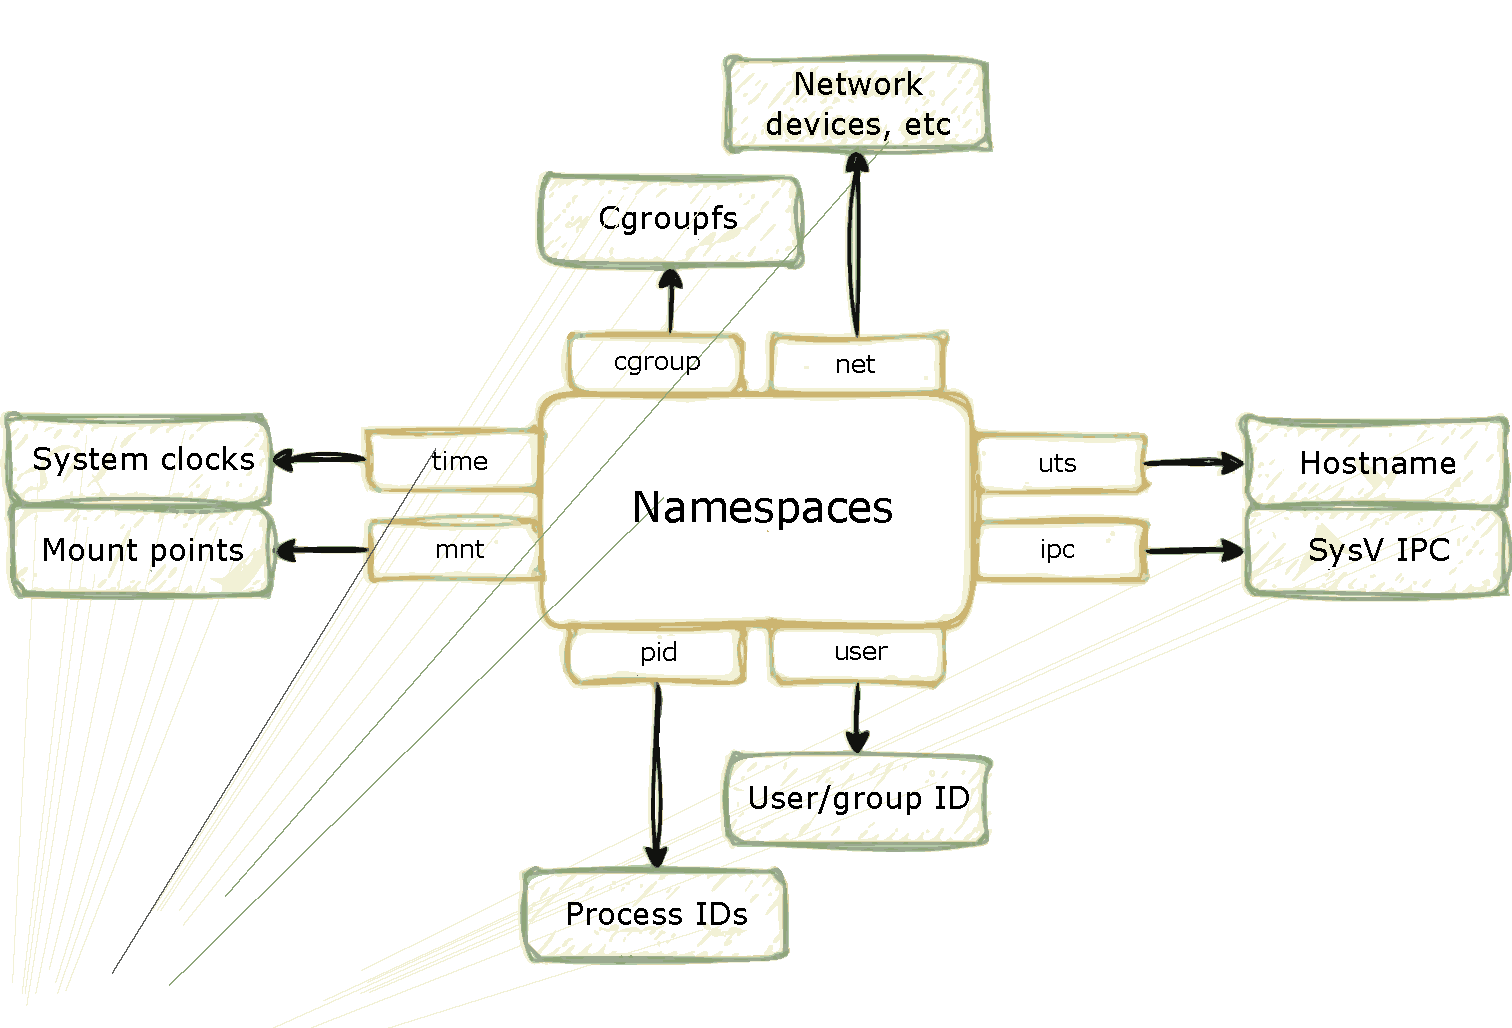
\includegraphics[width=0.8\textwidth]{figs/linux-namespaces-types.pdf}
  \figsource{\getauthor{hackerstack_namespaces}, \gettitle{hackerstack_namespaces} (\getyear{hackerstack_namespaces})~\cite{hackerstack_namespaces}.}
  \caption{Tipos de \textit{Namespaces}.}
  \label{fig:namespaces_types}
\end{figure}

Para lograr este nivel de flexibilidad, el \textit{kernel} no aplica un aislamiento monolítico sobre todo el sistema operativo de una única vez.
En su lugar, proporciona una arquitectura modular basada en distintos \textbf{tipos de \textit{Namespaces}}.
Cada tipo se encarga de aislar un recurso global específico, permitiendo a los administradores (o a los atacantes) crear combinaciones de los mismos de forma independiente según la finalidad de su uso~\cite{man_namespaces}.\\

Estos son los principales tipos de \textit{Namespaces} a implementar en un sistema \textit{Linux} moderno:

\begin{itemize}
    \item \textbf{\textit{Mount} (\texttt{mnt}):} Aísla los puntos de montaje del sistema de ficheros (concepto directamente relacionado con la Figura \ref{fig:mounting_point}). Los procesos dentro de este \textit{Namespace} poseen su propia visión de la jerarquía de directorios (\textit{FHS}).
    Esto implica que montar o desmontar una unidad extraíble (como un dispositivo \textit{USB}) en este espacio aislado no afectará ni será visible para el resto del sistema anfitrión.
    \item \textbf{\textit{PID} (\texttt{pid}):} Proporciona una jerarquía de procesos independiente. Como se puso de ejemplo antes, permite que el primer proceso ejecutado en ese espacio reciba el \textit{PID} 1, 
    aislando por completo la visibilidad hacia fuera del \textit{Namespace}. De esta manera, se impide que los procesos internos a este espacio puedan interactuar con los procesos externos al mismo.
    \item \textbf{\textit{User} (\texttt{user}):} Aísla los identificadores de usuario (\textit{UID}) y de grupo (\textit{GID}).
    En este espacio se permite que un proceso tenga privilegios absolutos de \textit{root} (\textit{UID} 0) dentro del mismo, mientras que en el exterior siga siendo tratado y restringido como un usuario estándar sin privilegios.
    \item \textbf{\textit{Network} (\texttt{net}):} Virtualiza y aísla toda la pila de red del sistema. Cada \textit{Namespace} de este tipo posee sus propias interfaces de red (incluyendo su propio \textit{loopback}),
    puertos, direcciones \textit{IP}, reglas de \textit{firewall} y tablas de enrutamiento (\textit{iptables} o \textit{nftables}).
    \item \textbf{\textit{UTS} (\texttt{uts}):} Permite que un grupo de procesos tenga su propio nombre de máquina (\textit{hostname}) y nombre de dominio \textit{NIS}, de forma independiente al nombre real del servidor físico de la máquina.
    \item \textbf{\textit{IPC} (\texttt{ipc}):} Aísla los recursos de comunicación entre procesos, como las colas de mensajes (\textit{POSIX}), los segmentos de memoria compartida y los semáforos.
    Impide que un proceso de este espacio interfiera o intercepte los mensajes de procesos externos.
    \item \textbf{\textit{Cgroup} (\texttt{cgroup}):} Encapsula la vista del directorio raíz de los grupos de control (\textit{Control Groups}).
    Esto oculta la jerarquía de políticas y límites de recursos (como \textit{CPU} o memoria) establecidos por el \textit{kernel}, evitando que un proceso aislado los conozca o intente modificarlos.
    \item \textbf{\textit{Time} (\texttt{time}):} Aísla los relojes internos del sistema, especialmente el reloj de arranque (\textit{boot clock}) y el reloj monotónico (\textit{monotonic clock}).
    Esto permite que este espacio aislado tenga su propia línea temporal, lo cual es muy útil para migrar contenedores entre diferentes servidores físicos sin alterar su percepción del tiempo de actividad (\textit{uptime}).
  \end{itemize}

La combinación estratégica de estos bloques es, precisamente, el motor tecnológico que hace posible la existencia de tecnologías de virtualización modernas como los contenedores (\textit{Docker}),
cuya arquitectura típica se ilustra en la siguiente Figura \ref{fig:ns-docker}.

\begin{figure}[h!]
  \centering
  \scalebox{0.8}{\definecolor{dockerpanel}{RGB}{216, 228, 239}
\definecolor{dockerborder}{RGB}{92, 109, 128}
\definecolor{dockertext}{RGB}{24, 31, 39}
\definecolor{dockersubtle}{RGB}{242, 246, 250}

\begin{tikzpicture}[
  x=1cm,
  y=1cm,
  panel/.style={
    draw=dockerborder,
    fill=dockerpanel,
    rounded corners=0.22cm,
    line width=0.95pt
  },
  chip/.style={
    draw=dockerborder,
    fill=dockersubtle,
    rounded corners=0.10cm,
    line width=0.75pt,
    minimum height=0.56cm,
    inner xsep=3.2pt,
    inner ysep=1.5pt,
    font=\fontfamily{Inter-LF}\fontsize{7.4}{8.2}\selectfont,
    text=dockertext,
    align=center
  },
  title/.style={
    font=\fontfamily{Inter-LF}\bfseries\fontsize{11.6}{12.6}\selectfont,
    text=dockertext
  }
]

  \node[anchor=north] at (6.0, 7.75) {
\includegraphics[width=5.15cm]{figs/docker_logo_official_deep_blue.pdf}};

  \node[panel, minimum width=5.05cm, minimum height=1.54cm] (storage) at (6.0, 5.18) {};
  \node[title] at (6.0, 5.46) {Storage};
  \node[chip, minimum width=1.52cm] at (4.9, 4.83) {Device Mapper};
  \node[chip, minimum width=0.78cm] at (6.6, 4.83) {Btrfs};
  \node[chip, minimum width=0.68cm] at (7.7, 4.83) {Aufs};

  \node[panel, minimum width=4.95cm, minimum height=1.46cm] (namespaces) at (3.2, 3.38) {};
  \node[title] at (3.2, 3.66) {Namespaces};
  \node[chip, minimum width=0.48cm] at (1.48, 3.02) {PID};
  \node[chip, minimum width=0.56cm] at (2.34, 3.02) {MNT};
  \node[chip, minimum width=0.48cm] at (3.2, 3.02) {IPC};
  \node[chip, minimum width=0.48cm] at (4.06, 3.02) {UTS};
  \node[chip, minimum width=0.54cm] at (4.92, 3.02) {NET};

  \node[panel, minimum width=4.95cm, minimum height=1.46cm] (networking) at (8.8, 3.38) {};
  \node[title] at (8.8, 3.66) {Networking};
  \node[chip, minimum width=0.72cm] at (7.5, 3.02) {veth};
  \node[chip, minimum width=0.98cm] at (8.7, 3.02) {bridge};
  \node[chip, minimum width=1.10cm] at (10.1, 3.02) {iptables};

  \node[panel, minimum width=4.95cm, minimum height=1.46cm] (cgroups) at (3.2, 1.58) {};
  \node[title] at (3.2, 1.86) {Cgroups};
  \node[chip, minimum width=0.56cm] at (1.35, 1.22) {cpu};
  \node[chip, minimum width=0.90cm] at (2.35, 1.22) {cpuset};
  \node[chip, minimum width=1.02cm] at (3.65, 1.22) {memory};
  \node[chip, minimum width=0.94cm] at (4.95, 1.22) {device};

  \node[panel, minimum width=4.95cm, minimum height=1.46cm] (security) at (8.8, 1.58) {};
  \node[title] at (8.8, 1.86) {Security};
  \node[chip, minimum width=1.02cm] at (7.4, 1.22) {Capability};
  \node[chip, minimum width=0.88cm] at (8.9, 1.22) {SELinux};
  \node[chip, minimum width=1.00cm] at (10.3, 1.22) {seccomp};
\end{tikzpicture}
}
  \figsource{Elaboración propia a partir de \getauthor{docker_overview}, \gettitle{docker_overview} (\getyear{docker_overview})~\cite{docker_overview}, usando el logotipo oficial de Docker~\cite{docker_brand}.}
  \caption{Ejemplo de arquitectura \textit{Docker}.}
  \label{fig:ns-docker}
\end{figure}

Todas estas tecnologías de aislamiento y abstracción, desde la gestión de memoria de la propia máquina hasta los \textit{Namespaces}, residen y se gestionan en el núcleo del sistema operativo.
Sin embargo, pese a su robustez, el \textit{kernel} no es una entidad monolítica e inalterable.
Para dotarlo de una alta flexibilidad y permitir la extensión de sus funcionalidades en tiempo real (o la alteración maliciosa de su comportamiento), este dispone de una arquitectura dinámica que permite inyectar y cargar código con máximos privilegios, como se explicará en el siguiente apartado.

\

\

\subsection{Módulos del Kernel de \textit{Linux} (\textit{LKMs})}
\label{sec:lkms}

Un \textbf{Módulo del Kernel} (\textit{LKM}) es código objeto compilado (cuyo código fuente está escrito en lenguaje \textit{C}) que puede ser cargado y descargado del espacio de memoria del núcleo (\textit{kernel}) en tiempo de ejecución.
Estos módulos permiten al \textit{kernel} extender sus funcionalidades (como incorporar nuevos sistemas de ficheros) sin necesidad de reiniciar el sistema ni recompilar el \textit{kernel} completo~\cite{geeks_lkm}.\\

El desarrollo de \textit{LKMs} presenta diferencias drásticas frente a la programación convencional en \textit{Espacio de Usuario}.
Al operar directamente en el nivel de máximos privilegios, los módulos no pueden acceder a la biblioteca estándar de \textit{C} (\texttt{libc}) y, por consiguiente, a funciones típicas como \texttt{printf()} o \texttt{malloc()}.
Además de esto, al formar parte del propio \textit{kernel}, tampoco pueden utilizar llamadas al sistema (\textit{syscalls}) a través de la interfaz estándar, sino que invocan directamente las funciones internas del \textit{kernel}.\\

Por otro lado, no existe una salida estándar por consola como ocurre en \textit{Espacio de Usuario}, y para suplirla, el \textit{kernel} proporciona su propia macro de impresión de \textit{logs}: \texttt{printk()}.
Las trazas generadas mediante esta función se almacenan en un \textit{buffer} circular interno y se registran en ficheros, típicamente en \texttt{/var/log/kern.log}.
Asimismo, \texttt{printk()} exige clasificar cada traza con un nivel de prioridad (\textit{log level}), abarcando eventos críticos o de error (\texttt{KERN\_EMERG} y \texttt{KERN\_ERR}), como también informativos o de depuración (\texttt{KERN\_INFO} y \texttt{KERN\_DEBUG}).\\

En cuanto a su compilación, se requieren las cabeceras del \textit{kernel} (paquetes \texttt{linux-headers}) que coincidan con la versión exacta del sistema.
Mediante un fichero \texttt{Makefile}, el código se compila generando un fichero objeto especial empaquetado con extensión \texttt{.ko} (\textit{Kernel Object}).
Una vez compilado, la gestión de su ciclo de vida se resume en cuatro fases básicas:

\begin{itemize}
    \item \textbf{\texttt{insmod}:} Inserción del código en \textit{Espacio de kernel}.
    \item \textbf{\texttt{modinfo}:} Reporte de los metadatos y dependencias del módulo.
    \item \textbf{\texttt{dmesg}:} Inspección de las trazas de ejecución del \textit{kernel}.
    \item \textbf{\texttt{rmmod}:} Extracción del módulo y liberación de los recursos de memoria.
\end{itemize}

\begin{code}[h!]
\begin{lstlisting}[language=bash]
# 0. Compilado del modulo mediante el fichero Makefile
$ make
make -C /lib/modules/6.12.41-current-bcm2711/build M=/home/lkms modules
make[1]: Entering directory '/usr/src/linux-headers-6.12.41-current-bcm2711'
  CC [M]  /home/lkms/hw.o
  MODPOST /home/lkms/Module.symvers
  CC [M]  /home/lkms/hw.mod.o
  LD [M]  /home/lkms/hw.ko
make[1]: Leaving directory '/usr/src/linux-headers-6.12.41-current-bcm2711'

# 1. Cargar el modulo (.ko) en el kernel
$ sudo insmod hw.ko

# 2. Inspeccionar los metadatos del modulo
$ modinfo hw.ko
filename:       /home/lkms/hw.ko
version:        0.1
description:    A simple Hello world LKM
author:         Noel Rodriguez Perez
license:        GPL
srcversion:     2F2B1B95DA1F08AC18B09BC
depends:        
vermagic:       6.12.41-current-bcm2711 SMP mod_unload modversions

# 3. Consultar las trazas generadas por printk
$ dmesg

# 4. Descargar el modulo liberando sus recursos
$ sudo rmmod hw
\end{lstlisting}
\caption[Comandos básicos de gestión de LKMs]{Comandos básicos para la gestión de un \textit{LKM}.}
\label{cod:lkm_commands}
\end{code}

A nivel de código fuente, la estructura lógica de cualquier \textit{LKM} se asienta sobre dos funciones principales.
En primer lugar, una \textbf{función de inicialización o de carga} (\texttt{module\_init()}), la cual se ejecuta automáticamente al insertar el módulo en el \textit{kernel} (mediante \texttt{insmod}) y se encarga de reservar los recursos necesarios o crear los ficheros virtuales implicados.
En segundo lugar, una \textbf{función de limpieza o de descarga} (\texttt{module\_exit()}), invocada al eliminar el módulo cargado (\texttt{rmmod}) con el fin de liberar la memoria utilizada y evitar fugas o estados inconsistentes en el sistema.\\

Finalmente, para poder establecer un canal o interfaz de comunicación bidireccional entre el \textit{Espacio de Usuario} y el \textit{Espacio del Kernel}, una de las técnicas más eficientes es la creación de ficheros virtuales a través del pseudo-sistema de ficheros de \textbf{\texttt{/proc}}.
De esta manera, el módulo instancia un fichero virtual (por ejemplo, \texttt{/proc/mydev}) y define manejadores personalizados (\textit{handlers}) que interceptan las llamadas al sistema que actúan sobre él, como \texttt{read} o \texttt{write}, y así poder declarar específicamente cómo interactuar con el \textit{Espacio de Usuario}.
Para implementar esta metodología en el \textit{LKM}, se precisa del uso de funciones específicas de la \textit{API} del \textit{kernel} que aseguran su correcto funcionamiento de forma segura, como \texttt{copy\_to\_user()} y \texttt{copy\_from\_user()} para la transferencia de información entre espacios de memoria distintos~\cite{medium_proc}.\\

En conclusión, el conjunto de todas las características estructurales y funcionales expuestas anteriormente constituye la base tecnológica de un sistema operativo \textit{Linux}.
Como se ha comentado previamente, este ha sido el entorno de trabajo elegido para desarrollar este proyecto, el cual se ha desplegado sobre una máquina física independiente y controlada.
Esto permite garantizar un acceso directo a las capas más profundas del sistema operativo, como el \textit{kernel} y sus módulos, mitigando cualquier riesgo sobre máquinas de producción o uso real.

\

\

\subsection{Entorno de desarrollo}
\label{sec:denv}

Teniendo en cuenta todas las funcionalidades descritas en entornos \textit{Linux}, se eligió realizar el desarrollo de este proyecto sobre una máquina física dedicada \textbf{Raspberry Pi 4 Model B} de \textbf{4 GB de RAM}, perteneciente a la familia de arquitecturas \textit{ARM}.
La elección de esta plataforma y de un sistema basado en \textit{Linux} se debe principalmente a su versatilidad y al alto grado de control que ofrece sobre el sistema operativo, el \textit{kernel} y las herramientas de bajo nivel necesarias para compilar, cargar y depurar \textit{Módulos del Kernel}.
Además, al tratarse de una máquina física aislada, se reducen los riesgos asociados a las pruebas con código en \textit{Espacio de Kernel}, evitando corromper un equipo de uso cotidiano y facilitando una experimentación más segura sobre un entorno real~\cite{rpi4_specs}.\\

\begin{figure}[h!]
  \centering
  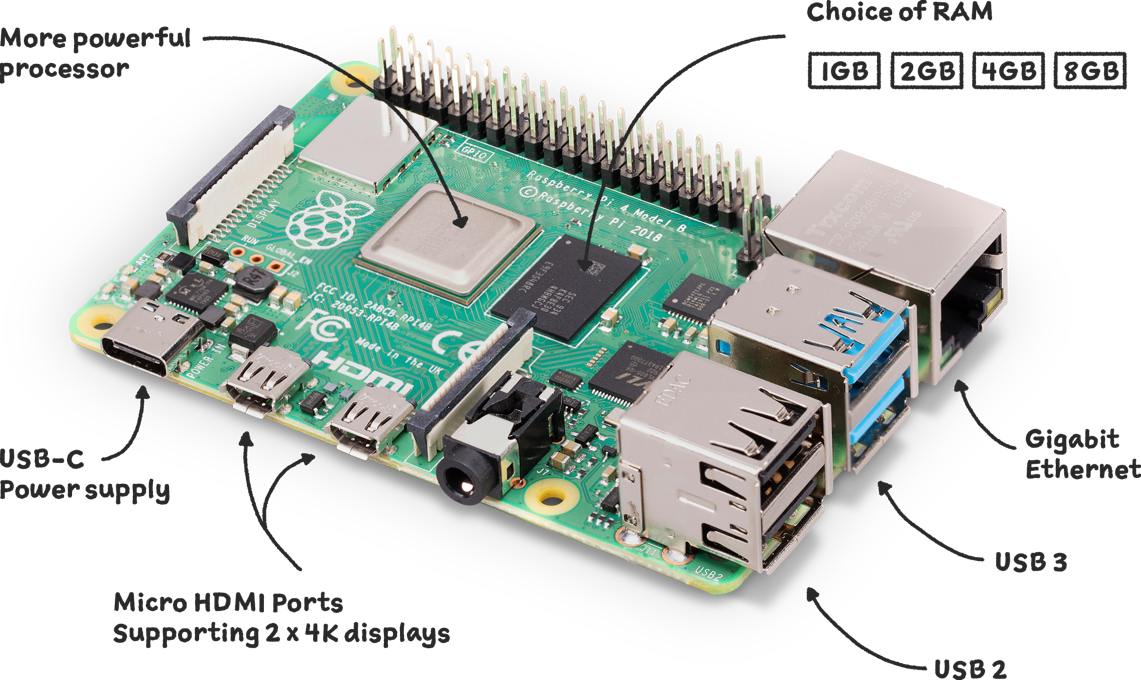
\includegraphics[width=0.65\textwidth]{figs/raspberry_pi.png}
  \figsource{Imagen oficial de Raspberry Pi 4 Model B~\cite{rpi4_product}.}
  \caption{Sistema físico empleado en el proyecto.}
  \label{fig:dev_pc}
\end{figure}

Sobre esta placa se instaló la distribución \textbf{Armbian}, en concreto una imagen para Raspberry Pi 4 basada en \textit{Ubuntu Noble}, orientada a placas \textit{single-board computer} y optimizada para arquitecturas \textit{ARM}.
Su elección se debe a que proporciona un entorno configurable, ligero y especialmente adecuado para este tipo de dispositivos, manteniendo al mismo tiempo la comodidad que ofrecen entornos \textit{Ubuntu}/\textit{Debian} y el gestor de paquetes \texttt{apt}~\cite{armbian_intro, armbian_rpi4b}.\\

\begin{figure}[h!]
  \centering
  
\includegraphics[width=0.35\textwidth]{figs/armbiam.pdf}
  \figsource{Imagen oficial de Armbian~\cite{armbian_brand}.}
  \caption{Logo de la distribución Armbian para Raspberry Pi 4 Model B.}
  \label{fig:armbian}
\end{figure}

Y por otro lado, la preparación del entorno comenzó con la instalación externa de dicha imagen de la distribución \textit{Armbian} en una tarjeta \textit{microSD} de 32 \textit{GB} y el arranque inicial de la placa tras introducirla.
Una vez iniciado el sistema, se actualizó y se instalaron las herramientas necesarias para la compilación en \textit{C} (\texttt{gcc} y \texttt{make}), el desarrollo de \textit{Módulos del Kernel} (\texttt{kmod}) y las cabeceras del \textit{kernel} necesarias para su compilación (\texttt{linux-headers}),
el uso de \textit{OpenSSL} (\texttt{openssl} y \texttt{libssl-dev}) y el despliegue de contenedores para crear nuevos espacios de nombres con \textit{Docker} (\texttt{docker.io}).

\begin{code}[h!]
\begin{lstlisting}[language=bash]
$ uname -r
6.12.41-current-bcm2711

$ sudo apt update
$ sudo apt install gcc make linux-headers-$(uname -r) \
>   kmod openssl libssl-dev docker.io
\end{lstlisting}
\caption[Instalación del entorno de desarrollo]{Instalación del entorno de desarrollo en \textit{Armbian} basado en \textit{Ubuntu Noble}.}
\label{cod:dev_env_install}
\end{code}

\newpage

Establecida la base tecnológica de los sistemas \textit{Linux} y definido el entorno de desarrollo, a continuación se presentará formalmente el problema de seguridad que explotan amenazas como los \textit{rootkits} y se plantearán los requisitos e implementaciones para la solución propuesta.
